\chapter{Konzeption der Softwarelösung}
\label{chap:konzeption_der_softwareloesung}

\section{Machine Learning Modell} \label{sec:06:machine_learning_model}

\subsection{XML-RoBERTa-large}

%TODO: https://huggingface.co/FacebookAI/xlm-roberta-large

\subsubsection{Cross-lingual Language Model (XML)}

In Kapitel \ref{sec04:bert} wurde bereits die Funktionsweise des MLMs erklärt. Kurz gefasst werden hierbei Wörter im Text zufällig maskiert, damit das Modell 
diese anschließend als Training erraten muss. BERT basiert auf diesem Ansatz. Die Erweiterung von MLM ist das Translation Language Model (TLM).
Im TLM werden statt einzelner Sätze (wie im MLM) übersetzte Satzpaare verwendet. Wörter in beiden Sprachen werden maskiert, und das Modell lernt, 
sie mithilfe beider Sprachversionen zu erraten (siehe Abbildung \ref{fig:translation_language_modeling}). So lernt es, die Bedeutungen über Sprachgrenzen hinweg zu 
verbinden.

\begin{figure}[htbp]
    \begin{center}
    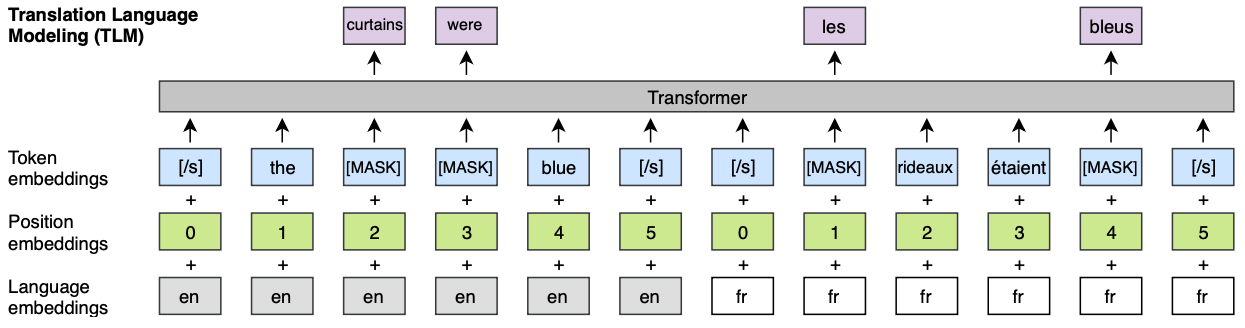
\includegraphics[scale=0.32]{static/translation_language_modeling.png}
    \caption{\label{fig:translation_language_modeling} Auswertung eines bilingualen Satzpaares von TLM \cite{NEURIPS2019_c04c19c2}}
    \end{center}
\end{figure}

XLM ist ein mehrsprachiges Sprachmodell, das darauf ausgelegt ist, Sprachverständnis über mehrere Sprachen hinweg zu ermöglichen.
Vortrainiert wird es mit MLM und zusätzlich TLM.
Durch diese Kombination kann das Modell lernen, ähnliche Inhalte in verschiedenen Sprachen miteinander zu verknüpfen \cite{NEURIPS2019_c04c19c2}.

\subsubsection{Sentence Piece Tokenizer} \label{subsec:sentencepiece}

Im Vergleich zum BERT Modell, welches den Word Piece Tokenizer nutzt, muss XML-RoBERTa den Sentence Piece Tokenizer nutzen. Dieser arbeitet sprachunabhängig, benötigt
keine vorab segmentierten Daten und funktioniert auch auf rohem Unicode-Text. 
Besonders wichtig ist das Konzept der Lossless Tokenization, das Segmentierung vollständig reversibel macht \cite{kudo-richardson-2018-sentencepiece}.
Sentence Piece setzt sich aus vier Hauptkomponenten zusammen. Dem Normalizer, Trainer, Encoder und Decoder. 

\begin{enumerate}
    \item Der \textbf{Normalizer} wandelt unter anderem alle Zeichen in ASCII um, normalisiert Leerzeichen und ersetzt alle Groß- mit Kleinbuchstaben.
    \item Der \textbf{Trainer} erstellt aus diesen normalisierten Daten daraufhin ein Subwort-Modell. Jedes Subwort bekommt eine eindeutige ID.
    \textless s \textgreater markiert den Start eines Satzes und hat immer die ID 0. Das \_ steht für ein Leerzeichen und markiert somit den Wortanfang.
    \item Der \textbf{Encoder} kodiert nun einen übergebenen Input basierend auf dem erstellten Subwort-Modell in eine ID-Sequenz.
    item Der \textbf{Decoder} dekodiert eine erstellte ID-Sequenz zurück in einen lesbaren Input.
\end{enumerate}

\subsubsection{conll2003 Datensatz}

%TODO: https://huggingface.co/datasets/eriktks/conll2003

\subsection{Datenvorverarbeitung}

RoBERTa lernt den Kontext der verschiedenen Artikel. Dafür müssen möglichst viele Informationen erhalten bleiben. 
Wie in Kapitel \ref{subsec:sentencepiece} beschrieben, erstellt RoBERTa analog zu BERT sein eigenes Word Embedding.

Der FNDG Datensatz enthält die Merkmale 'id', 'url', 'Titel', 'Body', 'Kategorie', 'Datum', 'Quelle', 'Fake' und 'Art'.
Hiervon beinhalten die drei Merkmale 'Titel', 'Body' und 'Fake' die relevanten Informationen für diese Anwendung.
In 'Titel' steht die jeweilige Überschrift des Artikels und in 'Body' der eigentliche Inhalt. Das Merkmal 'Fake' gibt in der Nominalskala
an ob der Artikel als gefälscht klassifiziert ist oder nicht (1 für Fake, 0 für echt).

Im FANG-COVID Datensatz sind die Merkmale 'Unnamed: 0.1', 'Unnamed: 0', 'article', 'date', 'header', 'label', 'url', 'hist', 'tweeet', 'repl', 'retw', 'like' und 'quote'
enthalten. 'article', 'header' und 'label' sind hierbei relevant. 'header' und 'article' sind analog zum FNDG Datensatz Überschrift und Inhalt
des Artikels. 'label' enthält entweder den Wert 'real' um den Artikel als echt oder 'fake' um den Artikel als gefälscht zu klassifizieren.

Die beiden Datensatze werden zur Weiterverarbeitung zusammengefasst. Überschrift und Inhalt werden konkateniert, da das RoBERTa Modell nur
einen Wert pro Label verarbeiten kann. Dieses Merkmal wird umbenannt zu 'text'. 
Für die Klassifizierungskennzeichnung wird die Nominalskala des FNDG Datensatzes und der Titel des FANG-Covid Datensatzes übernommen.

Danach folgt die Aufteilung der Daten in Trainings-, Validierungs- und Testdatensätze. 
80\% des Gesamtdatensatzes werden für das Training genutzt und jeweils 10\% für das Validierung und Testen.




\subsection{RoBERTa Model fine-tuning}

RoBERTa bietet viele bereits vortrainierte Modelle an. Diese sind unüberwacht trainiert worden. 


\subsection{LightGBM Model Training}

\subsection{Gesamtarchitektur}

\section{Hauptkomponente} \label{sec:06:hauptkomponente}

Die Hauptkomponente hat die Aufgabe die Artikel auf den verschiedenen Nachrichtenportalen zu lesen und zu ergänzen.
Hierfür muss erkannt werden auf welcher Seite sich der Nutzer befindet. Außerdem muss das html dieser Seite ausgelesen und analysiert werden können.

\paragraph{Als Beispiel die Seite Bild.de:} 
Je nach Fenstergröße hat die Seite entweder die Domäne \textit{https://www.bild.de/} oder \textit{https://m.bild.de/}.

Die Startseite ist wie folgt aufgebaut:

\begin{lstlisting} [language=html]
    <!DOCTYPE html>
    <html>
      <head>
        ...
      </head>
      <body>
        <div id="app">
            ...
            <div id="page-content">
                <header/>
                    <main>
                    <!-- Es gibt auf der Startseite 
                    ueber 50 dieser section-Elemente -->
                        <section>
                            <article/>
                        </section>
                    </main>
                <footer/>
            </div>    
        </div>
      </body>
    </html>
\end{lstlisting}

Wenn ein Artikel geöffnet ist, ist der DOM dem der Startseite sehr ähnlich. Der einzige wesentliche Unterschied ist, dass im \textit{main}-Element
nur noch ein \textit{article}-Element ist und nicht beliebig viele \textit{section}-Elemente.
Ob ein Artikel geöffnet ist, kann also anhand der Anzahl der \textit{article}-Elemente bestimmt werden.

\begin{lstlisting} [language=html]
    <article>
        <h2 class="document-title document-title-article">
            <span class="kicker">Kicker des Artikels</span>
            <span class="headline">Titel des Artikels</span>
        </h2>
    </article>
    <div class="article-body">
        <!-- Pro Artikel gibt es ca. 10 p-Elemente -->
        <p>Inhalt des Artikels</p>
    </div>
\end{lstlisting}

Der Titel und Inhalt des Artikels kann den entsprechenden html-Elementen entnommen werden.
Diese werden dann an die API gesendet und dort verarbeitet. 
Der Rückgabewert der API enthält dann die Info ob der Artikel falsch oder echt ist.
Diese wird in einem von der Hauptkomponente erzeugten \textit{div}-Container über dem Artikel eingefügt.

\begin{table}[ht]
    \centering
    \renewcommand{\arraystretch}{1.3}
    \begin{tabular}{|p{2.5cm}|p{2.5cm}|p{2.5cm}|p{2.5cm}|p{2.5cm}|}
        \hline
        \textbf{Kriterium} & \textbf{Chrome Extension} & \textbf{Userscript (Tampermonkey)} & \textbf{Proxy-Server} & \textbf{Scraper + Plattform} \\
        \hline
        DOM-Zugriff beim Nutzer & Ja & Ja & Nein & Nein \\
        \hline
        Einbindung auf \texttt{bild.de} direkt & Ja & Ja & Ja (indirekt) & Nein \\
        \hline
        Installation durch Nutzer & Mittel & Einfach & Nicht erforderlich & Nicht erforderlich\\
        \hline
        Komplexität der Umsetzung & Mittel & Gering & Hoch & Mittel \\
        \hline
        Wartbarkeit \& Updates & Gut & Gut & Aufwändig & Mittel \\
        \hline
        Performance beim Nutzer & Hoch & Hoch & Hoch & Hoch \\
        \hline
        Skalierbarkeit & Hoch & Eingeschränkt & Mittel & Hoch \\
        \hline
        Für öffentliche Verbreitung geeignet & Ja & Eingeschränkt & Eingeschränkt & Ja \\
        \hline
        API-Nutzung zur Fake-Erkennung & Ja & Ja & Ja & Ja \\
        \hline
        Entwickler-kontrolle über UI & Hoch & Mittel & Hoch & Mittel \\
        \hline
    \end{tabular}
    \caption{Vergleich verschiedener technischer Umsetzungsansätze}
    \label{table:technischeAnsaetze}
\end{table}

Zur Bestimmung des geeignetsten Tools um diese Anforderungen umzusetzen wurden verschiedene Umsetzungsansätze verglichen (siehe \ref{table:technischeAnsaetze}).
Aufgrund des begrenzten Zugriffs auf die zu analysierende Seiten, bieten sich die beiden Client-seitigen Umsetzungen 
eine Chrome Extension zu implementieren oder über Tampermonkey Userscripts auszuführen am ehesten an.

Im Vergleich zu Usercripts unterstützt die Extension mehrere Komponenten (Content Scripts, Background Scripts, Popup, Optionsseite).
Anhand dieser können der DOM beobachtet, ein persistenter Speicher genutzt, Kontextmenüs erstellt und auf Browseraktionen reagiert werden (z.B. Tabwechsel, Navigation).
Ein Userscript hingegen ist ein einfaches Script, das nur beim Laden einer Seite aktiv ist und dementsprechend keine Hintergrundverarbeitung und keine erweiterten UI-Komponenten
zur Verfügung stellt.

Zur Implementierung der Hauptkomponente wird also eine Chrome Extension genutzt.

    
    
    